\documentclass[tikz,border=8pt]{standalone}
% Shared look for every TikZ diagram. Load with \input{../../tools/tikz-style.tex}
\usepackage[T1]{fontenc}
\usepackage{lmodern}
\renewcommand{\sfdefault}{lmr}  % diagrams use the same serif as the text
\usetikzlibrary{arrows.meta, positioning, shapes.geometric, calc, fit, backgrounds}
\definecolor{cblue}{HTML}{4C78A8}
\definecolor{corange}{HTML}{F58518}
\definecolor{cgreen}{HTML}{54A24B}
\definecolor{cred}{HTML}{E45756}
\definecolor{cpurple}{HTML}{B279A2}
\definecolor{cgrey}{HTML}{6B6B6B}
\tikzset{
  every picture/.style={font=\sffamily, line width=1.2pt},
  box/.style={draw=#1, fill=#1!12, rounded corners=4pt, align=center, inner sep=7pt, minimum height=1.1cm},
  box/.default=cgrey,
  arrow/.style={-{Stealth[length=3mm]}, draw=cgrey, line width=1.4pt},
  title/.style={font=\sffamily\bfseries\Large},
  note/.style={font=\sffamily\small, text=cgrey, align=center},
}
\AtBeginDocument{\hyphenpenalty=10000 \exhyphenpenalty=10000}

% stack of #3 planes of side #2 (cm) at x=#1, colour #4; label #5 below, label #6 above
\newcommand{\planes}[6]{
  \foreach \k in {#3,...,1}{
    \fill[#4!14, draw=#4, line width=0.8pt] ({#1+(\k-1)*0.07},{-#2/2+(\k-1)*0.07}) rectangle ++(#2,#2);
  }
  \node[below, align=center] at ({#1+#2/2},{-1.75}) {#5};
  \node[above, align=center, font=\sffamily\small, text=cgrey] at ({#1+#2/2},{1.75}) {#6};
}
\newcommand{\layerbar}[5]{% vertical bar of nodes at x=#1, height #2, colour #3, label #4 below, #5 above
  \fill[#3!14, draw=#3, line width=0.8pt] (#1,-#2/2) rectangle ++(0.35,#2);
  \node[below, align=center] at (#1+0.175,-1.75) {#4};
  \node[above, align=center, font=\sffamily\small, text=cgrey] at (#1+0.175,1.75) {#5};
}
\begin{document}
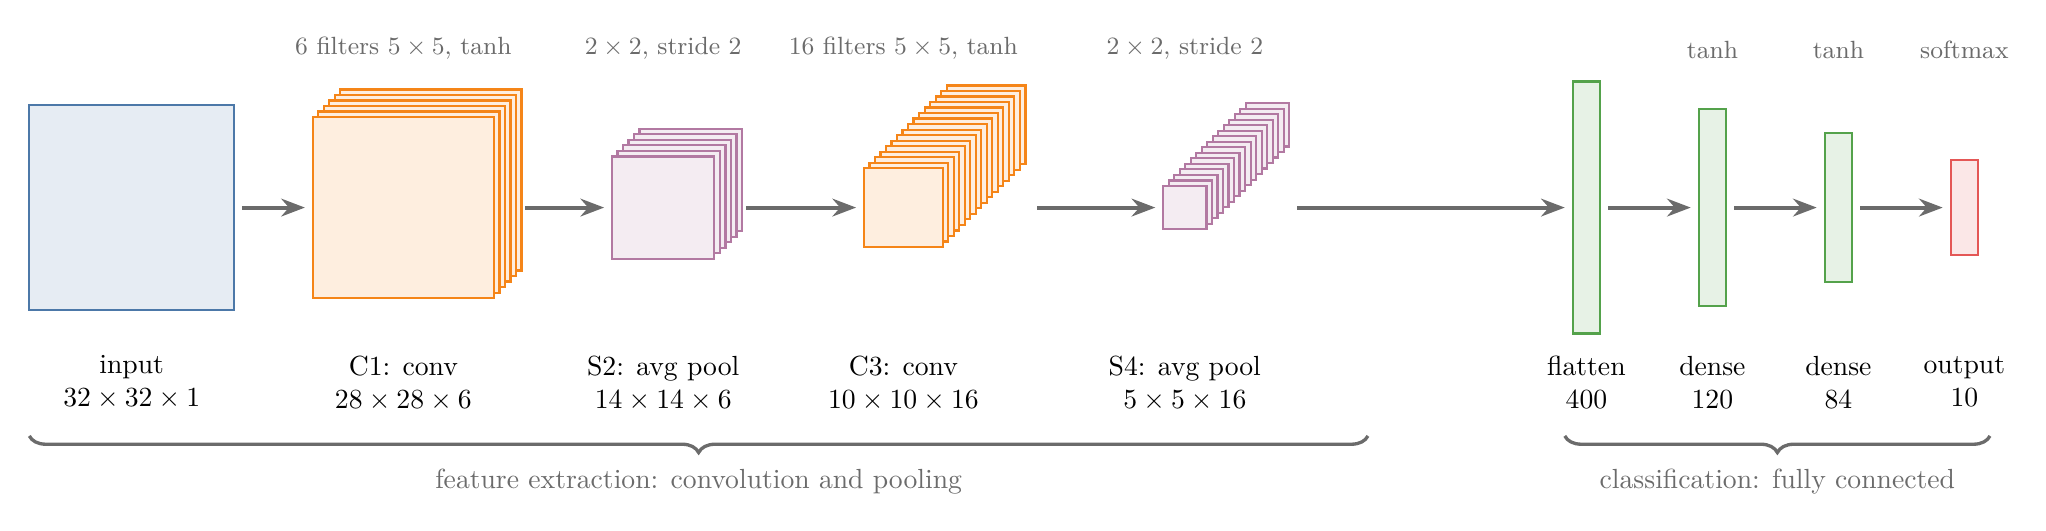
\begin{tikzpicture}[every node/.append style={font=\sffamily}]
  \planes{0}{2.6}{1}{cblue}{input\\$32 \times 32 \times 1$}{}
  \planes{3.6}{2.3}{6}{corange}{C1: conv\\$28 \times 28 \times 6$}{6 filters $5 \times 5$, tanh}
  \planes{7.4}{1.3}{6}{cpurple}{S2: avg pool\\$14 \times 14 \times 6$}{$2 \times 2$, stride 2}
  \planes{10.6}{1.0}{16}{corange}{C3: conv\\$10 \times 10 \times 16$}{16 filters $5 \times 5$, tanh}
  \planes{14.4}{0.55}{16}{cpurple}{S4: avg pool\\$5 \times 5 \times 16$}{$2 \times 2$, stride 2}
  \layerbar{19.6}{3.2}{cgreen}{flatten\\400}{}
  \layerbar{21.2}{2.5}{cgreen}{dense\\120}{tanh}
  \layerbar{22.8}{1.9}{cgreen}{dense\\84}{tanh}
  \layerbar{24.4}{1.2}{cred}{output\\10}{softmax}
  \foreach \a/\b in {2.7/3.5, 6.3/7.3, 9.1/10.5, 12.8/14.3, 16.1/19.5, 20.05/21.1, 21.65/22.7, 23.25/24.3}
    \draw[arrow] (\a,0) -- (\b,0);
  \draw[decorate, decoration={brace, amplitude=6pt, mirror}, cgrey] (0,-2.9) -- (17.0,-2.9)
     node[midway, below=8pt, text=cgrey] {feature extraction: convolution and pooling};
  \draw[decorate, decoration={brace, amplitude=6pt, mirror}, cgrey] (19.5,-2.9) -- (24.9,-2.9)
     node[midway, below=8pt, text=cgrey] {classification: fully connected};
\end{tikzpicture}
\end{document}
